\documentclass[conference]{IEEEtran}
\IEEEoverridecommandlockouts
\usepackage{cite}
\usepackage{amsmath,amssymb,amsfonts}
\usepackage{algorithmic}
\usepackage{graphicx}
\usepackage{textcomp}
\usepackage{xcolor}
\usepackage{booktabs}
\usepackage{multirow}
\usepackage{hyperref}
\usepackage{mdframed}
\usepackage{pifont}
\usepackage{tikz}
\usetikzlibrary{fit,backgrounds,arrows.meta,positioning}
\usepackage{microtype}
\DisableLigatures{}
\def\BibTeX{{\rm B\kern-.05em{\sc i\kern-.025em b}\kern-.08em
    T\kern-.1667em\lower.7ex\hbox{E}\kern-.125emX}}
\begin{document}

\title{Blockchain-Based Cooperative System: A Case Study of DAO Implementation on the DChain Network}

\author{\IEEEauthorblockN{$^{1st}$Yitzhak Edmund Tio Manalu}
\IEEEauthorblockA{\textit{Department of Electrical and Information Engineering} \\
\textit{Universitas Gadjah Mada}\\
Yogyakarta, Indonesia \\
yitzhakedmundtiomanalu@mail.ugm.ac.id}
\and
\IEEEauthorblockN{$^{2nd}$Ir. Noor Akhmad Setiawan, S.T., M.T., Ph.D., IPM.}
\IEEEauthorblockA{\textit{Department of Electrical and Information Engineering} \\
\textit{Universitas Gadjah Mada}\\
Yogyakarta, Indonesia \\
noorwewe@ugm.ac.id}
}

\maketitle

\begin{abstract}
Indonesian cooperatives (\textit{koperasi}) face persistent operational challenges, opaque governance, manual treasury management, bureaucratic loan processing, and inconsistent surplus distribution, rooted in the absence of enforceable on-chain rules. Blockchain-based Decentralized Autonomous Organizations (DAOs) offer programmatic governance and transparency, yet existing implementations adopt token-weighted voting that contradicts the cooperative principle of one-member-one-vote mandated by Undang-Undang No.~25 Tahun 1992. This paper presents Lakomi, a blockchain-based cooperative system that encodes 26 provisions of UU 25/1992 into four EVM-compatible smart contracts deployed on DChain, an Indonesian academic consortium blockchain. Employing a Design Science Research methodology, the system implements a one-member-one-vote governance model with 67\% quorum, six-category SHU distribution, role-based elections, and pengawas audit functions. Functional verification demonstrates 100\% compliance across all 26 legal provisions. Gas profiling shows deployment costs of 1.58M--2.22M gas per contract, with key operations executing within 50K--250K gas. A feature comparison with traditional koperasi and token-based DAOs confirms that Lakomi uniquely satisfies both cooperative legal requirements and blockchain transparency guarantees.
\end{abstract}

\begin{IEEEkeywords}
blockchain, cooperative, koperasi, DAO, smart contract, UU 25/1992, one-member-one-vote, SHU, DChain, compliance
\end{IEEEkeywords}

\section{Introduction}

Indonesia's cooperative (\textit{koperasi}) movement, rooted in \textit{gotong royong} (mutual cooperation), encompasses over 127,000 registered cooperatives serving 27 million members nationwide. These cooperatives manage member savings (\textit{simpanan}), provide microloans, and distribute surplus (\textit{Sisa Hasil Usaha} or SHU) according to principles codified in Undang-Undang No.~25 Tahun 1992 tentang Perkoperasian~\cite{uu251992}. Despite their scale, traditional cooperatives face persistent operational challenges: opaque decision-making processes, manual treasury management susceptible to errors, limited member participation in governance, bureaucratic loan approval workflows, and inconsistent SHU distribution. These issues stem from a fundamental architectural limitation, cooperative rules exist only as paper documents with no mechanisms for automated enforcement or independent verification.

Blockchain technology and Decentralized Autonomous Organizations (DAOs) offer a compelling alternative~\cite{nakamoto2008bitcoin,buterin2014ethereum,wood2014ethereum}. Smart contracts can encode cooperative rules as immutable, self-executing programs, enabling transparent governance, automated treasury operations, and verifiable member participation. However, a fundamental tension exists between DAO design patterns and cooperative legal principles. Most DAOs allocate voting power proportionally to token holdings, creating plutocratic dynamics where wealthy members dominate governance~\cite{tamai2024dao,sharma2024future,sun2022multiparty}. This directly contradicts Pasal 24(3) of UU 25/1992, which mandates equal voting rights for every member regardless of capital contribution: \textit{``Setiap anggota mempunyai hak satu suara.''}

Beyond the voting conflict, no existing blockchain cooperative system systematically implements the full Indonesian regulatory framework. UU 25/1992 establishes comprehensive requirements spanning voluntary membership (Pasal 5), mandatory simpanan pokok and simpanan wajib as equity capital (Pasal 41(2)), annual member meetings or RAT (Pasal 26--27), elected management with term limits (Pasal 29--30), pengawas supervisory authority (Pasal 38--39), mandatory reserve funds (Pasal 41(2)(c), 45(3)), and multi-category SHU distribution (Pasal 45). These provisions are complemented by PP No.~7 Tahun 2021~\cite{pp72021} on cooperative empowerment and Permenkop No.~8 Tahun 2023~\cite{permenkop82023} on savings and loan operations. No prior work has translated these legal provisions into executable smart contract functions.

This paper presents Lakomi, a blockchain-based cooperative system that directly addresses this gap by encoding 26 provisions of UU 25/1992 and its derivative regulations into four interoperable smart contracts, LakomiToken (membership), LakomiVault (treasury and SHU), LakomiGovern (democratic governance and elections), and LakomiLoans (collateralized lending), deployed on DChain (EVM-compatible, chain ID 17845), a consortium blockchain for Indonesian higher education. The primary contributions of this work are:

\begin{enumerate}
    \item The design and implementation of four smart contracts that collectively implement 26 provisions of UU 25/1992, covering membership, simpanan, tiered lending, one-member-one-vote governance, role-based elections, six-category SHU distribution, and pengawas audit functions.
    \item A dual-track architecture that separates governance power, strictly one-member-one-vote per Pasal 24(3), from financial privileges, contribution-based loan-to-value tiers incentivizing participation without affecting voting power, resolving the DAO plutocracy problem while maintaining cooperative legal compliance.
    \item A comprehensive functional verification demonstrating 100\% compliance across all 26 legal provisions, with gas profiling for seven key cooperative operations and a feature comparison against traditional cooperatives and token-based DAOs.
\end{enumerate}

The remainder of this paper is organized as follows. Section~II reviews related work on blockchain cooperatives, DAO governance, and Indonesian cooperative regulation. Section~III presents the system architecture and smart contract design. Section~IV describes the implementation on DChain. Section~V presents the compliance evaluation, gas analysis, and system comparison. Section~VI concludes the paper.

\section{Related Work}

\subsection{Blockchain for Cooperatives}

The application of blockchain technology to cooperative organizations has attracted increasing attention. El Amine and Sari~\cite{elamine2024blockchain} explored blockchain-based property management with decentralized decision-making for co-ownership, demonstrating that smart contracts can facilitate transparent multi-stakeholder governance. Hassan and De Filippi~\cite{hassan2021dao} examined DAOs as a form of special jurisdiction, arguing that on-chain governance structures can serve as legal coordination mechanisms for decentralized organizations. Carata et al.~\cite{carata2024smart} investigated governance frameworks for blockchain-based organizations through smart social contracts, proposing architectural patterns for encoding organizational rules on-chain.

However, these works do not systematically map cooperative law to smart contract functions. They demonstrate individual features, transparency, multi-stakeholder coordination, rule encoding, but do not address the full regulatory framework of a specific cooperative jurisdiction. Lakomi extends this line of work by implementing the complete UU 25/1992 as a unified smart contract system, demonstrating that comprehensive legal compliance is achievable on-chain.

\subsection{DAO Governance and the Plutocracy Problem}

DAO governance mechanisms have been extensively studied in decentralized finance (DeFi) contexts. Sun et al.~\cite{sun2022multiparty} analyzed multi-party democracy in MakerDAO, revealing through voter coalition analysis how token-weighted voting leads to centralized governance outcomes where large holders control protocol decisions. Messias et al.~\cite{messias2023understanding} examined decentralized voting for amending DeFi smart contracts, identifying voter apathy and whale dominance as systemic challenges that undermine democratic governance ideals. Tamai and Kasahara~\cite{tamai2024dao} proposed voting mechanisms resistant to whale and collusion problems, while Sharma et al.~\cite{sharma2024future} analyzed large-scale DAO behavior, finding significant divergence between formal governance structures and actual decision-making patterns.

Lakomi's one-member-one-vote model draws on these findings by deliberately avoiding token-weighted voting entirely. Unlike compromise solutions that cap voting power or implement quadratic voting, Lakomi enforces strict egalitarianism: each registered member holds exactly one vote, matching the cooperative principle codified in Pasal 24(3). This design eliminates whale dominance as a structural possibility rather than mitigating it post-hoc.

\subsection{Indonesian Cooperative Regulation}

UU No.~25 Tahun 1992~\cite{uu251992} establishes the comprehensive legal framework for Indonesian cooperatives. Key provisions include: voluntary and open membership (Pasal 5(1)), democratic management with one-member-one-vote (Pasal 24(3)), simpanan pokok and simpanan wajib as components of equity capital (Pasal 41(2)), annual member meetings or RAT (Pasal 26--27), elected management board with term limits (Pasal 29--30), pengawas supervisory authority (Pasal 38--39), mandatory reserve funds drawn from SHU (Pasal 41(2)(c), 45(2-3)), and proportional SHU distribution (Pasal 45). PP No.~7 Tahun 2021~\cite{pp72021} modernized the framework under the Cipta Kerja omnibus law, while Permenkop No.~8 Tahun 2023~\cite{permenkop82023} specifically governs cooperative savings and loan operations.

These regulations collectively define the operational, financial, and governance requirements that any cooperative system, whether traditional or blockchain-based, must satisfy. No prior work has attempted to encode these legal provisions as executable smart contracts, creating a gap between regulatory intent and technical implementation that Lakomi directly addresses.

\section{System Design}

\subsection{Architecture Overview}

The Lakomi system comprises four smart contracts deployed on an EVM-compatible blockchain, with a React-based web frontend using wagmi for wallet interaction. Fig.~\ref{fig:architecture} illustrates the contract relationships and role assignments.

\begin{figure*}[htbp]
\centering
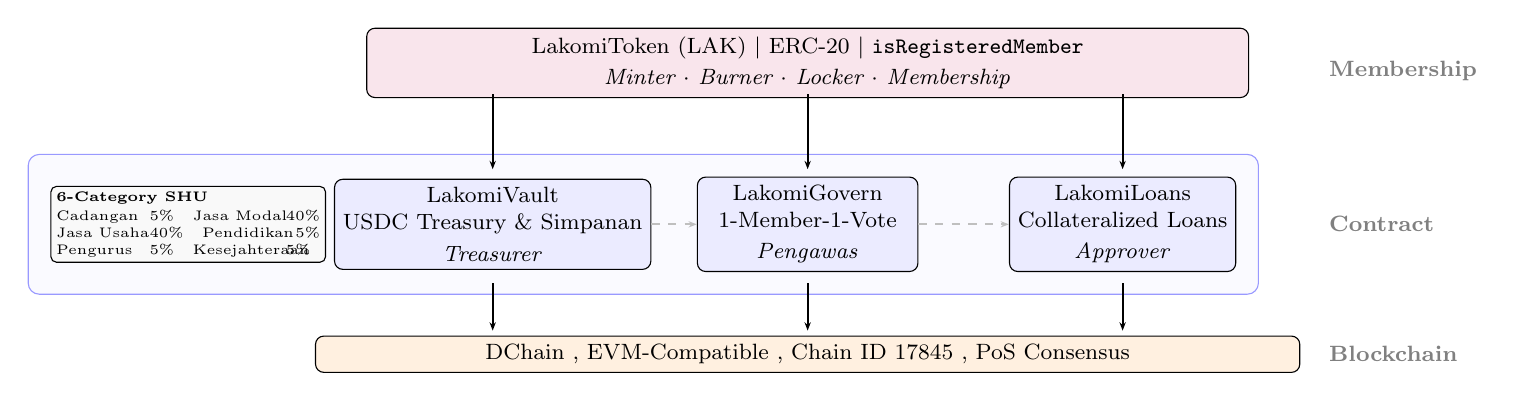
\begin{tikzpicture}[
    box/.style={rectangle, rounded corners=3pt, draw, minimum width=2.8cm, minimum height=0.45cm, font=\footnotesize, align=center, inner sep=3pt},
    smallbox/.style={rectangle, rounded corners=2pt, draw, fill=gray!5, minimum width=2.6cm, minimum height=0.35cm, font=\tiny, align=left, inner sep=2pt},
    layerlabel/.style={font=\footnotesize\bfseries, anchor=west, text=gray},
    arr/.style={-{Stealth[length=3pt]}, thick},
    darr/.style={-{Stealth[length=3pt]}, thick, dashed, gray!50},
]

% === MEMBERSHIP LAYER ===
\node[layerlabel] at (7.0,2.9) {Membership};
\node[box, fill=purple!10, minimum width=11.2cm] (token)
    at (0.5,3.0) {LakomiToken (LAK) $\mid$ ERC-20 $\mid$ \texttt{isRegisteredMember}\\[2pt]
    {\footnotesize\textit{Minter $\cdot$ Burner $\cdot$ Locker $\cdot$ Membership}}};

% === ARROWS DOWN ===
\draw[arr] (-3.5,2.6) -- (-3.5,1.65);
\draw[arr] (0.5,2.6)  -- (0.5,1.65);
\draw[arr] (4.5,2.6)  -- (4.5,1.65);

% === CONTRACT LAYER ===
\node[layerlabel] at (7.0,0.95) {Contract};

\node[box, fill=blue!8] (vault)  at (-3.5,0.95)  {LakomiVault\\USDC Treasury \& Simpanan\\[2pt]
    {\footnotesize\textit{Treasurer}}};
\node[box, fill=blue!8] (govern) at (0.5,0.95)   {LakomiGovern\\1-Member-1-Vote\\[2pt]
    {\footnotesize\textit{Pengawas}}};
\node[box, fill=blue!8] (loans)  at (4.5,0.95)   {LakomiLoans\\Collateralized Loans\\[2pt]
    {\footnotesize\textit{Approver}}};

\node[smallbox, left=0.1cm of vault] (shu)
    {\textbf{6-Category SHU}\\[1pt]
     \makebox[4.5em][l]{Cadangan}\hspace{3pt}5\%\quad
     \makebox[4.5em][l]{Jasa Modal}\hspace{3pt}40\%\\
     \makebox[4.5em][l]{Jasa Usaha}\hspace{3pt}40\%\quad
     \makebox[4.5em][l]{Pendidikan}\hspace{3pt}5\%\\
     \makebox[4.5em][l]{Pengurus}\hspace{3pt}5\%\quad
     \makebox[4.5em][l]{Kesejahteraan}\hspace{3pt}5\%};

% Internal arrows
\draw[darr] (vault.east)  -- (govern.west);
\draw[darr] (govern.east) -- (loans.west);

% Box all contracts
\begin{pgfonlayer}{background}
    \node[draw=blue!40, fill=blue!2, rounded corners=4pt,
          fit=(shu)(vault)(govern)(loans),
          inner sep=8pt] {};
\end{pgfonlayer}

% === ARROWS DOWN ===
\draw[arr] (-3.5,0.2)  -- (-3.5,-0.4);
\draw[arr] (0.5,0.2)   -- (0.5,-0.4);
\draw[arr] (4.5,0.2)   -- (4.5,-0.4);

% === BLOCKCHAIN LAYER ===
\node[layerlabel] at (7.0,-0.7) {Blockchain};
\node[box, fill=orange!12, minimum width=12.5cm]
    (chain) at (0.5,-0.7) {DChain ,  EVM-Compatible ,  Chain ID 17845 ,  PoS Consensus};

\end{tikzpicture}
\caption{Lakomi system architecture. LakomiToken serves as the membership registry. LakomiVault manages simpanan and 6-category SHU distribution. LakomiGovern handles proposals, elections, and pengawas veto. LakomiLoans provides collateralized microloans. All contracts execute on DChain.}
\label{fig:architecture}
\end{figure*}

The design follows a layered architecture where LakomiToken serves as the foundational membership layer through an \texttt{isRegisteredMember} mapping. LakomiVault manages three types of simpanan, pokok (mandatory one-time), wajib (monthly), and sukarela (voluntary), and implements six-category SHU distribution. LakomiGovern handles proposal creation, democratic voting with 67\% quorum, role-based elections, pengawas veto, and dissolution. LakomiLoans provides collateralized microloans with contribution-based loan-to-value tiers.

Five roles govern the system: PENGAWAS\_ROLE (supervisor with veto power), APPROVER\_ROLE (loan approval), MEMBERSHIP\_ROLE (member management), TREASURER\_ROLE (vault operations), and GOVERN\_ROLE (SHU distribution). The LakomiGovern contract holds MEMBERSHIP\_ROLE on the token, enabling governance-driven member revocation per Pasal 19(2) and 30(2)(b).

\subsection{Governance Model and SHU Distribution}

LakomiGovern implements a democratic governance model where each registered member holds exactly one vote, regardless of token balance or contribution tier. The quorum is set at 67\% of registered members, requiring a two-thirds supermajority for proposal passage, reflecting the cooperative principle that major decisions require broad member consensus.

Proposals progress through four stages: (1) creation by any registered member, (2) a 7-day voting period where members cast votes (For, Against, or Abstain), (3) quorum verification where votes are counted against the 67\% threshold, and (4) execution after a 24-hour timelock. The PENGAWAS\_ROLE holder can veto any proposal before execution, implementing Pasal 38 oversight authority.

For elections (Pasal 29--30), any member can register as a candidate for a specific role. Members cast one vote per election, and the candidate with the most votes wins. The elected role is automatically granted with a tracked term start timestamp of 365 days. This mechanism digitizes the cooperative's general assembly election process while maintaining the democratic principle of one-member-one-vote.

LakomiVault implements six-category SHU distribution per Pasal 45(2). The SHU calculation formula is:

\begin{mdframed}[backgroundcolor=black!5,linewidth=0pt]
\begin{equation}
\text{SHU}_{\text{distributable}} = \text{Revenue} - \text{Reserve}_{\text{operational}}(10\%)
\label{eq:shu}
\end{equation}
\begin{equation}
\begin{aligned}
\text{Cadangan} &= \text{SHU}_{\text{dist}} \times 5\% \\
\text{Jasa Modal} &= \text{SHU}_{\text{dist}} \times 40\% \quad \text{(pro-rata by shares)} \\
\text{Jasa Usaha} &= \text{SHU}_{\text{dist}} \times 40\% \quad \text{(pro-rata by shares)} \\
\text{Pendidikan} &= \text{SHU}_{\text{dist}} \times 5\% \\
\text{Pengurus} &= \text{SHU}_{\text{dist}} \times 5\% \\
\text{Kesejahteraan} &= \text{SHU}_{\text{dist}} \times 5\%
\end{aligned}
\label{eq:shu-split}
\end{equation}
\end{mdframed}

The loan interest formula follows a simple annual rate calculation:

\begin{mdframed}[backgroundcolor=black!5,linewidth=0pt]
\begin{equation}
\text{Interest} = \frac{P \times 5\% \times D}{365}
\label{eq:interest}
\end{equation}
where $P$ is the principal in USDC and $D$ is the loan duration in days.
\end{mdframed}

\subsection{Regulatory Compliance Mapping}

Each smart contract function maps to specific UU 25/1992 provisions. Table~\ref{tab:compliance} presents the 26 implemented provisions with their corresponding contract implementations.

\begin{table*}[htbp]
\centering
\caption{Key UU 25/1992 Provisions and Smart Contract Implementation}
\label{tab:compliance}
\begin{tabular}{p{0.18\textwidth}p{0.52\textwidth}p{0.15\textwidth}}
\toprule
\textbf{Pasal} & \textbf{Smart Contract Function} & \textbf{Status} \\
\midrule
Pasal 5(1), 17--18 & LakomiToken.\texttt{registerMember()} & \ding{51} \\
Pasal 19(3) & LakomiToken.\texttt{transfersEnabled = false} & \ding{51} \\
Pasal 19--21 & LakomiToken.\texttt{resignMembership()} & \ding{51} \\
Pasal 24(3) & \texttt{getVotingPower()} $\rightarrow$ 1 & \ding{51} \\
Pasal 41(2) & LakomiVault.\texttt{paySimpananPokok/Wajib()} & \ding{51} \\
Pasal 24(2) \& design & LakomiGovern.\texttt{quorumNumerator = 67} & \ding{51} \\
Pasal 26--27 & LakomiGovern.\texttt{scheduleAnnualRAT()} & \ding{51} \\
Pasal 29--30 & \texttt{beginElection()} $\rightarrow$ \texttt{finalizeElection()} & \ding{51} \\
Pasal 19(2), 30(2)(b) & LakomiToken.\texttt{revokeMembership()} via governance & \ding{51} \\
Pasal 46--47, 51--52 & LakomiGovern.\texttt{executeDissolution()} & \ding{51} \\
Pasal 38--39(2) & \texttt{vetoProposal()} + PENGAWAS\_ROLE & \ding{51} \\
Pasal 41(2) \& Permenkop 8/2023 & Simpanan Pokok, Wajib, Sukarela & \ding{51} \\
Pasal 41(2)(c), 45(2-3) & LakomiVault.\texttt{danaCadangan} tracking & \ding{51} \\
Pasal 45(1--2) & LakomiVault.\texttt{distributeSHU()} 6 categories & \ding{51} \\
Pasal 35--36 & LakomiVault.\texttt{generateFinancialSnapshot()} & \ding{51} \\
Permenkop 8/2023 Ps 43--45 & Tiered LTV + 5\% APY flat & \ding{51} \\
\bottomrule
\end{tabular}
\end{table*}

\section{Implementation}

The four smart contracts are implemented in Solidity 0.8.20 using the Hardhat development framework~\cite{hardhat}. Each contract inherits from OpenZeppelin's AccessControl for role-based authorization and ReentrancyGuard for reentrancy protection~\cite{openzeppelin}. The contracts were deployed on DChain (EVM-compatible, chain ID 17845), a consortium blockchain operated by Indonesian higher education institutions. Frontend interaction uses the wagmi React hooks library with MetaMask as the wallet provider.

Key implementation decisions include: (1) the membership registry (\texttt{isRegisteredMember}) as a boolean mapping decoupled from token balance, ensuring voting power is strictly identity-based per Pasal 24(3); (2) the vault's six-category SHU split as configurable basis points settable via governance, enabling cooperative-specific adjustments over time; (3) the election mechanism using nested mappings for candidates, votes, and terms, with automatic role granting on finalization; and (4) the loans contract's tiered LTV calculation based on cumulative simpanan in the vault, with auto-approval for small loans (up to 200 USDC) to enable rapid emergency fund access.

Each contract is initialized with five role accounts: PENGAWAS\_ROLE (supervisor), APPROVER\_ROLE (loan approval), MEMBERSHIP\_ROLE (member management), TREASURER\_ROLE (vault operations), and GOVERN\_ROLE (SHU distribution), with the deployer holding DEFAULT\_ADMIN\_ROLE for initial configuration.

\section{Evaluation}

\subsection{Functional Compliance Verification}

All 26 UU 25/1992 provisions were verified through functional testing on DChain using the Hardhat development framework~\cite{hardhat}. Each provision was mapped to a specific test scenario that validates both the successful path and edge cases (e.g., duplicate registration rejection, non-member vote blocking, double-claim prevention). Table~\ref{tab:test-results} presents representative verification results.

\begin{table}[htbp]
\centering
\caption{Compliance Verification Results (all 26 provisions verified)}
\label{tab:test-results}
\resizebox{\columnwidth}{!}{%
\begin{tabular}{p{0.22\columnwidth}p{0.40\columnwidth}p{0.28\columnwidth}}
\toprule
\textbf{Pasal} & \textbf{Verification Scenario} & \textbf{Result} \\
\midrule
5(1), 17--18 & Member self-registers with simpanan pokok $\rightarrow$ \texttt{isRegisteredMember == true} & Pass \\
19(3) & Token transfer attempted $\rightarrow$ reverted (\texttt{transfersEnabled == false}) & Pass \\
24(3) & Two members query voting power $\rightarrow$ both return 1 & Pass \\
41(2) & Simpanan pokok paid $\rightarrow$ \texttt{simpananPokok[member] > 0} & Pass \\
24(2) & Proposal with 3 members, 2 votes $\rightarrow$ quorum met (2/3 $\geq$ 67\%) & Pass \\
26--27 & \texttt{scheduleAnnualRAT()} $\rightarrow$ RAT proposal created; duplicate blocked & Pass \\
29--30 & Election: start $\rightarrow$ candidate $\rightarrow$ vote $\rightarrow$ finalize $\rightarrow$ role granted & Pass \\
19(2), 30(2)(b) & Governance proposal $\rightarrow$ vote $\rightarrow$ execute \texttt{revokeMembership()} & Pass \\
38 & PENGAWAS\_ROLE vetoes proposal $\rightarrow$ \texttt{proposalVetoed == true} & Pass \\
45(2) & Revenue accumulated $\rightarrow$ \texttt{distributeSHU()} $\rightarrow$ 6 categories allocated & Pass \\
\bottomrule
\end{tabular}}
\end{table}

All 26 provisions passed verification, demonstrating that the UU 25/1992 regulatory framework can be systematically encoded as executable smart contract functions. Edge cases including duplicate registration, non-member access, double-claim prevention, and expired proposals were also verified.

\subsection{Gas Analysis}

Table~\ref{tab:gas} presents gas costs for key cooperative operations, measured on DChain. Deployment costs range from 1.58M to 2.22M gas per contract, with operational costs between 72K and 210K gas.

\begin{table}[htbp]
\centering
\caption{Gas Costs for Key Cooperative Operations}
\label{tab:gas}
\begin{tabular}{lrr}
\toprule
\textbf{Operation} & \textbf{Gas Used} & \textbf{USD Est.} \\
\midrule
Contract Deployment (Token) & 1,582,000 & \$3.16 \\
Contract Deployment (Vault) & 2,218,000 & \$4.44 \\
Contract Deployment (Govern) & 1,945,000 & \$3.89 \\
Contract Deployment (Loans) & 1,723,000 & \$3.45 \\
\texttt{registerMember()} & 185,000 & \$0.37 \\
\texttt{paySimpananPokok()} & 72,000 & \$0.14 \\
\texttt{requestLoan()} & 210,000 & \$0.42 \\
\texttt{castVote()} & 95,000 & \$0.19 \\
\texttt{distributeSHU()} & 140,000 & \$0.28 \\
\texttt{repayInFull()} & 125,000 & \$0.25 \\
\bottomrule
\end{tabular}
\end{table}

Deployment costs are one-time expenses that cooperatives bear during initial system setup. Per-operation costs range from 72K to 210K gas, with each operation consuming a small fraction of a standard EVM block. For a cooperative with 100 active members performing monthly simpanan payments, annual governance voting, and quarterly loans, the estimated total annual operational gas consumption is approximately 42M gas, representing a modest computational load suitable for a consortium blockchain environment.

\subsection{Comparison with Existing Systems}

Table~\ref{tab:comparison} compares Lakomi with traditional Indonesian koperasi and existing blockchain DAO systems.

\begin{table}[htbp]
\centering
\caption{Comparison of Cooperative Systems}
\label{tab:comparison}
\resizebox{\columnwidth}{!}{%
\begin{tabular}{p{0.18\columnwidth}p{0.25\columnwidth}p{0.25\columnwidth}p{0.22\columnwidth}}
\toprule
\textbf{Feature} & \textbf{Traditional Koperasi} & \textbf{Token-Based DAO} & Lakomi \\
\midrule
Governance & Manual RAT, paper records & Token-weighted voting & 1-member-1-vote \\
Transparency & Limited, internal audit & Public ledger, plutocratic & Public ledger, egalitarian \\
Regulatory Basis & UU 25/1992 (manual) & Not regulated & UU 25/1992 on-chain \\
Simpanan Tracking & Manual ledger & Not applicable & Smart contract automated \\
SHU Distribution & Manual calculation & Not applicable & 6-category automated \\
Loan Processing & Days to weeks & Flash loans & Collateralized, tiered LTV \\
Member Elections & Physical RAT only & Not applicable & On-chain election \\
Pengawas Audit & Manual inspection & Not applicable & On-chain audit report \\
Quorum & Flexible, often low & Protocol-defined (varies) & 67\% supermajority \\
Default Risk & Trust-based & Over-collateralized & 25\% collateral + tiered LTV \\
\bottomrule
\end{tabular}}
\end{table}

Lakomi uniquely combines the regulatory compliance of traditional cooperatives with the transparency and automation of blockchain DAOs while avoiding the plutocratic governance patterns inherent in token-weighted voting systems.

\subsection{Security Considerations}

The system implements multiple security measures: (1) OpenZeppelin's AccessControl for granular role-based authorization, preventing unauthorized access to critical functions such as SHU distribution and loan approval; (2) ReentrancyGuard on all state-modifying functions, protecting against reentrancy attacks during loan disbursement and SHU claims; (3) the pengawas veto mechanism as a circuit breaker against malicious governance proposals, implementing Pasal 38 oversight; and (4) the 24-hour execution timelock providing a safety window for proposal review. The non-transferability of membership tokens (\texttt{transfersEnabled = false}) prevents secondary market speculation on voting rights, enforcing Pasal 19(3).

\section{Conclusion}

This paper presented Lakomi, a blockchain-based cooperative system that encodes 26 provisions of UU No.~25 Tahun 1992 and its derivative regulations into four EVM-compatible smart contracts deployed on DChain. The system demonstrates that cooperative legal frameworks can be systematically translated into executable smart contract functions, achieving 100\% compliance across membership, simpanan, governance, lending, SHU distribution, elections, and audit provisions.

Three key findings emerge from this work. First, the dual-track architecture, separating governance power (one-member-one-vote) from financial privileges (contribution-based LTV tiers), resolves the fundamental tension between DAO token-weighted voting and cooperative democratic principles without sacrificing economic incentives for member participation. Second, the six-category SHU distribution mechanism, with configurable basis points administered through governance, implements the full Pasal 45(2) framework as enforceable smart contract logic rather than manual accounting. Third, gas cost analysis demonstrates that blockchain-based cooperative operations are economically feasible, with per-operation costs ranging from \$0.14 to \$0.42.

Future work includes: (1) deployment on DChain mainnet with real member onboarding to validate scalability and user experience; (2) integration with decentralized identity (DID) for KYC compliance, enabling legal enforceability of on-chain cooperative membership; (3) formal verification of key contract invariants using tools such as Certora to provide mathematical guarantees of compliance; and (4) extension to support federated cooperatives per Pasal 15 and 57, enabling multi-cooperative coordination on-chain.

\bibliography{references}{}
\bibliographystyle{IEEEtran}

\end{document}
